\section{积分与微分}
\label{sec:integral-differentiation}

卷一的微积分基本定理有两个方向：被积函数$g$连续时，累计函数$G(x)=\int_a^xg(t)\,\mathrm dt$可导且$G'=g$；$F$连续可导时，$F(b)-F(a)=\int_a^bF'(t)\,\mathrm dt$（可参考\BookChapterRef{chap:univariate-integration}{卷一“一元函数的积分”章}）。有了Lebesgue积分，被积函数只需可积，导数也只需几乎处处存在，两个方向都要重新回答：可积函数的累计函数在什么意义下可导，导数是否回到原函数？哪些函数能由导数的积分恢复？第二章的Cantor函数连续、单调，导数几乎处处为零，整体却从$0$增到$1$，可见“连续且几乎处处可导”不够。本节回到有限闭区间$[a,b]$上的实值函数，先定义控制多个区间总增量的绝对连续性，再用有界变差和区间覆盖得到导数的存在与总量估计，然后分别处理积分函数的求导和由导数恢复函数，最后用Cantor函数检查恢复公式的边界。全部论证只用一元函数和区间覆盖，不使用第四章的相对密度。

\subsection{绝对连续函数}
\label{sec:integral-absolutely-continuous}

\paragraph{从单个区间到多个区间}
一致连续要求：只要一个区间足够短，函数在它两端的增量就小。要由导数恢复增量，这还不够，因为导数为零的地方可能散布着许多极短的区间，函数恰好在这些区间上完成全部增长。需要控制的是许多互不相交的小区间上的总增量。

\begin{definition}[绝对连续函数]
\label{def:integral-absolutely-continuous-function}
设$F:[a,b]\to\mathbb R$。若对任意$\varepsilon>0$存在$\delta>0$，使得对$[a,b]$中任意有限个两两不交的开区间$(a_1,b_1),\ldots,(a_m,b_m)$，只要$\sum_{i=1}^m(b_i-a_i)<\delta$，就有
\[
 \sum_{i=1}^m|F(b_i)-F(a_i)|<\varepsilon,
\]
则称$F$在$[a,b]$上绝对连续，也称$F$是$[a,b]$上的\term{绝对连续函数}（absolutely continuous function）。
\end{definition}

取$m=1$就回到一致连续的要求，所以绝对连续函数一致连续。区别在于$\delta$必须对任意多个小区间同时有效：区间个数不受限制，只限制总长度。图~\ref{fig:integral-absolute-continuity-intervals}中取$F(x)=\sqrt x$，横轴上四段绿色区间总长$1.2$，纵轴上对应的四段红色增量总和约为$0.562$；绝对连续性要求，当绿色总长趋于零时，红色总和也一致地趋于零，无论区间怎样分布、分成多少段。

\begin{figure}[!htbp]
\centering
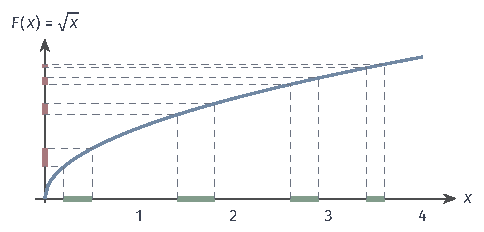
\includegraphics[width=81.933mm]{figures/02-abstract-mathematics/01-metric-and-measure/tikz/c3-absolute-continuity-intervals/figure.pdf}
\caption{绝对连续性控制的是多个不交区间上的总增量。$F(x)=\sqrt x$，纵轴放大$1.2$倍绘制。横轴上的绿色区间为$(0.2,0.5)$、$(1.4,1.8)$、$(2.6,2.9)$、$(3.4,3.6)$，总长$1.2$；纵轴上的红色线段是相应增量$0.260$、$0.158$、$0.090$、$0.053$，总和约为$0.562$。靠近原点的区间虽短，增量却最大。}
\label{fig:integral-absolute-continuity-intervals}
\end{figure}

\paragraph{基本例子与性质}
若$F$满足Lipschitz条件$|F(x)-F(y)|\le L|x-y|$，则$\sum_i|F(b_i)-F(a_i)|\le L\sum_i(b_i-a_i)$，取$\delta=\varepsilon/L$即可，所以Lipschitz函数绝对连续；特别地，$[a,b]$上连续可导的函数由中值定理满足Lipschitz条件，因而绝对连续。有限线性组合保持绝对连续：若$F,G$绝对连续、$\alpha,\beta\in\mathbb R$，对$\varepsilon$分别取$F,G$的$\delta_F,\delta_G$，使对应总增量小于$\varepsilon/(2|\alpha|+2|\beta|+1)$，令$\delta=\min(\delta_F,\delta_G)$，三角不等式给出$\alpha F+\beta G$的总增量小于$\varepsilon$。绝对连续函数不一定Lipschitz：$\sqrt x$在$[0,4]$上于原点附近斜率无界，却绝对连续，这一点在第~\ref{sec:integral-indefinite}小节可以直接看出。

这里的“绝对连续”描述的是函数增量受区间长度的控制，与第二章两个测度之间的绝对连续$\nu\ll\mu$（定义~\ref{def:measure-absolutely-continuous}）定义不同。两者怎样通过函数增量所确定的测度联系起来，留到第四章的密度计算中说明。

\subsection{有界变差与几乎处处可导}
\label{sec:integral-bounded-variation}

\paragraph{全变差}
要从导数读出函数的变化，先要确认变化的总量有限。

\begin{definition}[有界变差函数]
\label{def:integral-bounded-variation}
对$F:[a,b]\to\mathbb R$和$[a,b]$的分割$P:a=x_0<x_1<\cdots<x_n=b$，令$V(F,P)=\sum_{k=1}^n|F(x_k)-F(x_{k-1})|$。称
\[
 V_a^b(F)=\sup_PV(F,P)
\]
为$F$在$[a,b]$上的\term{全变差}（total variation）。若$V_a^b(F)<\infty$，称$F$为$[a,b]$上的\term{有界变差函数}（function of bounded variation）。
\end{definition}

函数的全变差是沿区间累计的增量绝对值，与第二章有符号测度的总变差测度$|\nu|$是不同的对象。单调函数的全变差就是端点增量$|F(b)-F(a)|$，因为每个分割上的和都可以伸缩相消。全变差对区间可加：若$a<c<b$，则$V_a^b(F)=V_a^c(F)+V_c^b(F)$。理由是在分割中插入点$c$不会减小$V(F,P)$（三角不等式），而插入$c$后的分割恰好分成$[a,c]$与$[c,b]$两部分的分割。

\begin{lemma}[绝对连续函数有界变差]
\label{lem:integral-ac-bv}
若$F$在$[a,b]$上绝对连续，则$F$是有界变差函数。
\end{lemma}

\begin{proof}
对$\varepsilon=1$取定义中的$\delta$。把$[a,b]$等分成$K$段，$K$取得足够大使每段长度小于$\delta$。在一段$[c,d]$内任取分割，其小区间两两不交、总长小于$\delta$，增量之和小于$1$，故$V_c^d(F)\le1$。由区间可加性，$V_a^b(F)\le K$。
\end{proof}

一致连续不能推出有界变差。在$[0,1]$上令$F(x)=x\sin(1/x)$（$x>0$）、$F(0)=0$，它在紧区间上连续，因而一致连续。取$x_k=1/((k+\frac12)\pi)$，则$F(x_k)=(-1)^kx_k$，相邻两点的增量绝对值为$x_k+x_{k+1}>x_k$，于是$V_0^1(F)\ge\sum_kx_k=\sum_k\frac1{(k+\frac12)\pi}=\infty$。由引理~\ref{lem:integral-ac-bv}，这个函数也不绝对连续。

有界变差函数总能写成两个单调函数之差。令$V(x)=V_a^x(F)$（$V(a)=0$），称为$F$的\term{变差函数}（variation function）。对$a\le x<y\le b$，由区间可加性，$V(y)-V(x)=V_x^y(F)\ge|F(y)-F(x)|$。因此$V$与$V-F$都单调不减，且
\[
 F=V-(V-F)
\]
是两个有限值单调不减函数之差。这一分解只用到函数本身，没有构造任何测度；它把有界变差函数的研究归结为单调函数。

\paragraph{单调函数的可导性}
单调函数可能在可数个点跳跃，也可能像Cantor函数那样在零测集上完成增长，但它在几乎每一点都有有限导数。证明的核心是一个区间选择引理。设$E\subseteq\mathbb R$，$\mathcal V$是一族非退化闭区间；若对每个$x\in E$和每个$\eta>0$，都有$I\in\mathcal V$满足$x\in I$且$|I|<\eta$，就称$\mathcal V$为$E$的\term{Vitali覆盖}（Vitali cover），其中$|I|$表示区间长度。

\begin{lemma}[Vitali覆盖引理]
\label{lem:integral-vitali}
设$E\subseteq\mathbb R$的外测度$\lambda^*(E)<\infty$，$\mathcal V$是$E$的Vitali覆盖。则对任意$\varepsilon>0$，存在$\mathcal V$中有限个两两不交的区间$I_1,\ldots,I_N$，使$\lambda^*\bigl(E\setminus\bigcup_{k=1}^NI_k\bigr)<\varepsilon$。
\end{lemma}

\begin{proof}
由外测度的定义（定义~\ref{def:measure-outer}），可以用可数个开区间覆盖$E$且总长不超过$\lambda^*(E)+1$，它们的并是开集$O\supseteq E$，$\lambda(O)<\infty$。只保留$\mathcal V$中含于$O$的区间；$O$是开集，每点附近的足够短的区间都含于$O$，所以剩下的仍是Vitali覆盖。

归纳地选取区间。设已选出两两不交的$I_1,\ldots,I_n$。若它们已覆盖$E$，结论成立；否则令
\[
 k_n=\sup\{|I|:I\in\mathcal V,\ I\text{与}I_1,\ldots,I_n\text{都不相交}\}.
\]
$E$中未被覆盖的点到闭集$I_1\cup\cdots\cup I_n$有正距离，它附近足够短的区间与已选区间都不相交，所以$k_n>0$；这些区间都含于$O$，所以$k_n\le\lambda(O)$。选取与已选区间不交的$I_{n+1}\in\mathcal V$，使$|I_{n+1}|>k_n/2$。所选区间两两不交，含于$O$，故$\sum_n|I_n|\le\lambda(O)<\infty$，从而$|I_n|\to0$，$k_n<2|I_{n+1}|\to0$。

取$N$使$\sum_{n>N}|I_n|<\varepsilon/5$。记$5I_n$为与$I_n$同心、长度为$5|I_n|$的闭区间。下面证明$E\setminus\bigcup_{k\le N}I_k\subseteq\bigcup_{n>N}5I_n$，于是其外测度不超过$5\sum_{n>N}|I_n|<\varepsilon$。任取该集合中的$x$，与上一段相同，存在$I\in\mathcal V$含$x$且与$I_1,\ldots,I_N$都不相交。$I$不能与全部$I_n$都不相交，否则$|I|\le k_n$对所有$n$成立，而$k_n\to0$与$|I|>0$矛盾。设$n$是使$I\cap I_n\ne\varnothing$的最小下标，则$n>N$，并且$I$与$I_1,\ldots,I_{n-1}$不交，故$|I|\le k_{n-1}<2|I_n|$。$x\in I$，$I$与$I_n$相交，所以$x$到$I_n$中点的距离不超过$|I|+|I_n|/2<\frac52|I_n|$，即$x\in5I_n$。
\end{proof}

图~\ref{fig:integral-vitali-cover}展示了最后一步的放大论证：未选中的区间$I$若碰到某个已选区间$I_n$，且长度不超过$I_n$的两倍，就整个落在$5I_n$之内。所以已选区间的五倍放大接住了所有漏掉的点，而尾部区间的总长任意小。

\begin{figure}[!htbp]
\centering
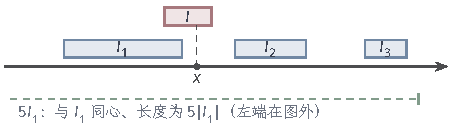
\includegraphics[width=76.616mm]{figures/02-abstract-mathematics/01-metric-and-measure/tikz/c3-vitali-cover/figure.pdf}
\caption{Vitali选择中的五倍放大。蓝色为已选的两两不交区间$I_1=[0.5,2.5]$、$I_2=[3.4,4.6]$、$I_3=[5.6,6.3]$；红色区间$I=[2.2,3.0]$含点$x$，与$I_1$相交且$|I|=0.8<2|I_1|$，因此落在与$I_1$同心、长为$5|I_1|=10$的区间$5I_1=[-3.5,6.5]$中（绿色虚线只画出右侧部分）。}
\label{fig:integral-vitali-cover}
\end{figure}

为描述导数可能不存在的情况，对$x\in(a,b)$引入四个\term{Dini导数}（Dini derivative）：
\[
 \begin{gathered}
 D^+F(x)=\limsup_{h\downarrow0}\frac{F(x+h)-F(x)}h,\\
 D_+F(x)=\liminf_{h\downarrow0}\frac{F(x+h)-F(x)}h,
 \end{gathered}
\]
$D^-F(x)$与$D_-F(x)$则分别是左侧差商$\bigl(F(x)-F(x-h)\bigr)/h$在$h\downarrow0$时的上极限与下极限。$F$在$x$处可导当且仅当四者相等且有限。对单调不减的$F$，四者都取值于$[0,\infty]$。

\begin{theorem}[单调函数几乎处处可导]
\label{thm:integral-monotone-differentiable}
设$F:[a,b]\to\mathbb R$单调不减。则$F$在$[a,b]$上几乎处处有有限导数，$F'$（在导数不存在处取$0$）Lebesgue可积，并且
\begin{equation}
 \int_a^bF'(x)\,\mathrm dx\le F(b)-F(a).
 \label{eq:integral-monotone-derivative-bound}
\end{equation}
\end{theorem}

\begin{proof}
先证明四个Dini导数几乎处处相等，这一步是补充阅读，读者可以先接受结论，直接看下一段的积分估计。取有理数$0<u<v$，令$E=\{x\in(a,b):D_-F(x)<u<v<D^+F(x)\}$，$s=\lambda^*(E)$。对$\varepsilon>0$取开集$O\supseteq E$，$\lambda(O)<s+\varepsilon$。每个$x\in E$都有任意小的$h>0$使$[x-h,x]\subseteq O\cap(a,b)$且$F(x)-F(x-h)<uh$；这些区间构成$E$的Vitali覆盖，由引理~\ref{lem:integral-vitali}选出两两不交的$[x_k-h_k,x_k]$（$k\le N$），未覆盖部分外测度小于$\varepsilon$，并且
\[
 \sum_{k=1}^N\bigl(F(x_k)-F(x_k-h_k)\bigr)<u\sum_kh_k\le u\lambda(O)<u(s+\varepsilon).
\]
令$A$为$E$落在这些区间内部的部分，则$\lambda^*(A)>s-\varepsilon$（端点只有有限个）。每个$y\in A$都有任意小的$k>0$，使$[y,y+k]$含于某个$(x_j-h_j,x_j)$且$F(y+k)-F(y)>vk$。再用引理选出两两不交的$J_1,\ldots,J_M$，未覆盖部分外测度小于$\varepsilon$，故$\sum_m|J_m|>s-2\varepsilon$，$F$在这些区间上的增量之和大于$v(s-2\varepsilon)$。每个$J_m$都在某个$[x_k-h_k,x_k]$内，$F$单调不减，同一个$[x_k-h_k,x_k]$内不交子区间上的增量之和不超过它两端的增量。于是$v(s-2\varepsilon)<u(s+\varepsilon)$。令$\varepsilon\to0$得$vs\le us$，而$v>u$，所以$s=0$。对所有有理数对取并，$\{D_-F<D^+F\}$零测，即$D^+F\le D_-F$几乎处处成立。把这一结论用于单调不减函数$\tilde F(x)=-F(-x)$（定义在$[-b,-a]$上），由$D^+\tilde F(x)=D^-F(-x)$、$D_-\tilde F(x)=D_+F(-x)$得到$D^-F\le D_+F$几乎处处成立。于是几乎处处有
\[
 D^+F\le D_-F\le D^-F\le D_+F\le D^+F,
\]
四者相等，$F$的导数在$[0,\infty]$中几乎处处存在。

再证明积分估计，它同时说明导数几乎处处有限。对$x>b$令$F(x)=F(b)$，并令$q_n(x)=n\bigl(F(x+1/n)-F(x)\bigr)$。单调函数的上水平集是区间，所以$F$与$q_n$可测；$q_n\ge0$，并且在导数存在处$q_n\to F'$。由Fatou引理（引理~\ref{lem:integral-fatou}），
\[
 \int_a^bF'\,\mathrm dx\le\liminf_{n\to\infty}\int_a^bq_n\,\mathrm dx.
\]
平移不改变Lebesgue积分（定理~\ref{thm:integral-jacobian-change}，平移的Jacobian因子为$1$），所以
\[
 \begin{aligned}
 \int_a^bq_n\,\mathrm dx&=n\int_{a+1/n}^{b+1/n}F-n\int_a^bF\\
 &=n\int_b^{b+1/n}F-n\int_a^{a+1/n}F\le F(b)-F(a),
 \end{aligned}
\]
最后一步用到$[b,b+1/n]$上$F=F(b)$、$[a,a+1/n]$上$F\ge F(a)$。这就是式~\eqref{eq:integral-monotone-derivative-bound}。左侧有限，可积的非负函数几乎处处有限，所以导数几乎处处有限。
\end{proof}

由$F=V-(V-F)$，有界变差函数是两个单调函数之差，因而也几乎处处可导，并且$|F'|\le V'+(V-F)'$几乎处处成立，导数绝对可积。结合引理~\ref{lem:integral-ac-bv}，绝对连续函数同样几乎处处可导，导数可积。

\paragraph{还没有得到的结论}
式~\eqref{eq:integral-monotone-derivative-bound}只是不等式，等号可以不成立。$[0,1]$上的阶跃函数$F=\mathbf 1_{[1/2,1]}$单调不减，除$x=1/2$外导数都是$0$，导数的积分为$0$，而$F(1)-F(0)=1$；增量全部发生在一个点上，导数读不到它。所以有界变差和导数可积只给出导数的存在与总量的上界，还不能说明导数的积分等于函数的增量。要排除导数读不到的变化，必须用到绝对连续性；在证明之前，不能把待证的微积分基本定理当作依据。

\subsection{积分函数的绝对连续性与导数}
\label{sec:integral-indefinite}

先看微积分基本定理的第一个方向。设$g$在$[a,b]$上Lebesgue可积，令
\[
 G(x)=\int_a^xg(t)\,\mathrm dt\qquad(a\le x\le b),
\]
这里$\int_a^x$表示在$[a,x]$上对$\lambda$积分。我们要证明$G$绝对连续，并且$G'=g$几乎处处成立。

\paragraph{积分函数绝对连续}
多个不交区间上$G$的增量之和不超过$|g|$在这些区间之并上的积分，所以需要的是：测度很小的集合上，$|g|$的积分也很小。

\begin{lemma}[积分的绝对连续性]
\label{lem:integral-small-sets}
设$g$关于$\mu$可积。则对任意$\varepsilon>0$存在$\delta>0$，使对每个满足$\mu(A)<\delta$的可测集$A$，都有$\int_A|g|\,\mathrm d\mu<\varepsilon$。
\end{lemma}

\begin{proof}
把$|g|$分成有界的截断$\min(|g|,n)$与尾部$|g|-\min(|g|,n)$。截断随$n$递增到$|g|$，单调收敛定理给出$\int\min(|g|,n)\,\mathrm d\mu\uparrow\int|g|\,\mathrm d\mu<\infty$，所以可取$n$使尾部的积分小于$\varepsilon/2$。令$\delta=\varepsilon/(2n)$。当$\mu(A)<\delta$时，
\[
 \int_A|g|\,\mathrm d\mu\le\int_A\min(|g|,n)\,\mathrm d\mu+\int\bigl(|g|-\min(|g|,n)\bigr)\,\mathrm d\mu<n\delta+\frac\varepsilon2=\varepsilon.
\]
\end{proof}

对$[a,b]$中两两不交的$(a_i,b_i)$，令$A=\bigcup_i(a_i,b_i)$，则
\[
 \sum_i|G(b_i)-G(a_i)|=\sum_i\Bigl|\int_{a_i}^{b_i}g\Bigr|\le\int_A|g|\,\mathrm d\lambda.
\]
总长$\lambda(A)<\delta$时右侧小于$\varepsilon$，所以$G$绝对连续。例如在$[0,4]$上取$g(t)=1/(2\sqrt t)$，它在原点附近无界，但$\int_0^4g=2$有限；$G(x)=\int_0^xg=\sqrt x$（对$[\eta,x]$用卷一的公式再令$\eta\downarrow0$，由单调收敛得到），因此$\sqrt x$绝对连续，这正是图~\ref{fig:integral-absolute-continuity-intervals}中的函数。

\paragraph{Lebesgue微分定理}
$G$绝对连续，由上一小节它几乎处处可导；剩下的问题是导数是否等于$g$。卷一的结论只在$g$的连续点处成立，而可积函数可以处处不连续，例如$[0,1]$上有理数的示性函数，它的积分函数恒为$0$，导数$0$与原函数只在零测的有理点上不同。下面的定理说明，“几乎处处”正是一般情形下的准确答案。

\begin{lemma}[区间积分全为零的函数]
\label{lem:integral-vanishing-intervals}
设$g$在$[a,b]$上可积且为实值。若对每个$x\in[a,b]$都有$\int_a^xg=0$，则$g=0$几乎处处成立。
\end{lemma}

\begin{proof}
改动零测集不影响结论，不妨设$g$是Borel函数。令$\mathcal D$为使$\int_Eg=0$的Borel集$E\subseteq[a,b]$全体。区间$(c,d]\subseteq[a,b]$满足$\int_{(c,d]}g=\int_a^dg-\int_a^cg=0$，这些区间和空集对有限交封闭，生成$[a,b]$上的Borel $\sigma$代数（单点也是零测的，可以并入）。$\mathcal D$是$\lambda$系统：$[a,b]\in\mathcal D$；补集由$\int_{E^c}g=\int g-\int_Eg$得到；两两不交的可数并由控制收敛定理（以$|g|$为控制）得到积分可数可加。由$\pi$--$\lambda$定理，$\mathcal D$包含全部Borel集。取$E=\{g>0\}$，得$\int g\mathbf 1_{\{g>0\}}=0$，非负函数积分为零，所以$g\le0$几乎处处成立；同理$g\ge0$几乎处处成立。
\end{proof}

\begin{theorem}[Lebesgue微分定理]
\label{thm:integral-lebesgue-differentiation}
设$g$在$[a,b]$上Lebesgue可积，$G(x)=\int_a^xg(t)\,\mathrm dt$。则$G$绝对连续，并且$G'=g$几乎处处成立，即对几乎每个$x\in(a,b)$，
\[
 \lim_{h\to0}\frac1h\int_x^{x+h}g(t)\,\mathrm dt=g(x).
\]
\end{theorem}

\begin{proof}
绝对连续性已经证明。复值情形对实部、虚部分别处理，实值情形由$g=g^+-g^-$与导数的线性性，只需对$g\ge0$证明。

先设$0\le g\le M$。此时$|G(y)-G(x)|\le M|y-x|$，$G$是Lipschitz函数，由上一小节它几乎处处可导。对$x>b$令$G(x)=G(b)$，差商$q_n(x)=n\bigl(G(x+1/n)-G(x)\bigr)$满足$|q_n|\le M$，并在$G$可导的点趋于$G'$。对$c\in(a,b]$，在$[a,c]$上以常数$M$为控制用控制收敛定理，再像定理~\ref{thm:integral-monotone-differentiable}的证明那样平移，得
\[
 \int_a^cG'\,\mathrm dx=\lim_{n\to\infty}\Bigl(n\int_c^{c+1/n}G-n\int_a^{a+1/n}G\Bigr)=G(c)-G(a),
\]
最后一步用到$G$连续，函数在缩小区间上的平均值趋于端点值。于是$\int_a^c(G'-g)=0$对所有$c$成立，由引理~\ref{lem:integral-vanishing-intervals}，$G'=g$几乎处处成立。

再看一般的$g\ge0$。令$g_n=\min(g,n)$，$G_n(x)=\int_a^xg_n$。由有界情形，$G_n'=g_n$几乎处处成立。$G-G_n=\int_a^x(g-g_n)$单调不减，其导数在几乎每点非负，所以$G'\ge G_n'=g_n$几乎处处成立；对可数个$n$合并例外集，得$G'\ge g$几乎处处成立。另一方面，$G$单调不减，由式~\eqref{eq:integral-monotone-derivative-bound}，
\[
 \int_a^bG'\le G(b)-G(a)=\int_a^bg.
\]
因此$G'-g\ge0$几乎处处成立且积分不超过$0$，故$G'=g$几乎处处成立。最后，$G'(x)=g(x)$按定义就是$\frac1h\bigl(G(x+h)-G(x)\bigr)=\frac1h\int_x^{x+h}g\to g(x)$。
\end{proof}

\term{Lebesgue微分定理}的名称来自最后一种表述：$g$在$x$附近的局部平均值，在几乎每一点恢复$g$的取值。常见的另一种证明先建立最大平均值函数的弱型估计，再用连续函数逼近可积函数；这里改用单调函数的可导性和上面的区间引理，二者都是一元区间上的论证，不需要后面的函数空间完备性，也不使用第四章的相对密度定理。

\subsection{微积分基本定理}
\label{sec:integral-ftc}

现在处理第二个方向：给定绝对连续的$F$，证明$F(x)-F(a)=\int_a^xF'$。由第~\ref{sec:integral-bounded-variation}小节，$F'$几乎处处存在且可积；令$G(x)=F(a)+\int_a^xF'(t)\,\mathrm dt$。由上一小节，$G$绝对连续且$G'=F'$几乎处处成立。于是$H=F-G$绝对连续，并且$H'=0$几乎处处成立。恢复公式就归结为：导数几乎处处为零的绝对连续函数必为常数。

\paragraph{零导数引理}
阶跃函数和Cantor函数说明，没有绝对连续性时这个结论不成立。绝对连续性的作用，是控制导数为零的点之外那些总长很小的间隙上的增量。

\begin{lemma}[零导数引理]
\label{lem:integral-zero-derivative}
若$H$在$[a,b]$上绝对连续，且$H'=0$几乎处处成立，则$H$是常数。
\end{lemma}

\begin{proof}
任取$c\in(a,b]$，证明$H(c)=H(a)$。给定$\varepsilon>0$，取绝对连续定义中的$\delta$。令$E=\{x\in(a,c):H'(x)=0\}$，则$\lambda(E)=c-a$。对每个$x\in E$，$H'(x)=0$保证有任意小的$h>0$，使$[x,x+h]\subseteq(a,c)$且$|H(x+h)-H(x)|<\varepsilon h$。这些区间构成$E$的Vitali覆盖。由引理~\ref{lem:integral-vitali}，可以选出两两不交的$[x_k,y_k]$（$k=1,\ldots,N$，按$x_1<y_1<x_2<\cdots<y_N$排列），使$\lambda\bigl(E\setminus\bigcup_k[x_k,y_k]\bigr)<\delta$。

记$y_0=a$、$x_{N+1}=c$。$[a,c]$去掉所选区间后剩下的间隙$(y_k,x_{k+1})$（$k=0,\ldots,N$）两两不交，总长不超过$\lambda\bigl(E\setminus\bigcup_k[x_k,y_k]\bigr)+\lambda([a,c]\setminus E)<\delta$。把端点增量沿选中区间和间隙拆开：
\[
 \begin{aligned}
 |H(c)-H(a)|&\le\sum_{k=1}^N|H(y_k)-H(x_k)|+\sum_{k=0}^N|H(x_{k+1})-H(y_k)|\\
 &<\varepsilon\sum_k(y_k-x_k)+\varepsilon\le\varepsilon(c-a+1).
 \end{aligned}
\]
前一项由导数为零控制，后一项由绝对连续性控制。$\varepsilon$任意，所以$H(c)=H(a)$。
\end{proof}

\paragraph{恢复公式与双向刻画}
零导数引理补上了最后一步。

\begin{theorem}[Lebesgue微积分基本定理]
\label{thm:integral-ftc}
设$F:[a,b]\to\mathbb R$。以下两条等价：
\begin{enumerate}
 \item $F$在$[a,b]$上绝对连续；
 \item 存在$[a,b]$上的Lebesgue可积函数$g$，使$F(x)=F(a)+\int_a^xg(t)\,\mathrm dt$对所有$x\in[a,b]$成立。
\end{enumerate}
此时$F$几乎处处可导，$F'=g$几乎处处成立，并且
\begin{equation}
 F(x)-F(a)=\int_a^xF'(t)\,\mathrm dt\qquad(a\le x\le b).
 \label{eq:integral-ftc}
\end{equation}
\end{theorem}

\begin{proof}
(2)推出(1)及$F'=g$几乎处处成立，就是定理~\ref{thm:integral-lebesgue-differentiation}。(1)推出(2)：如本小节开头所述，$F'$几乎处处存在且可积，$H=F-F(a)-\int_a^xF'$绝对连续且$H'=0$几乎处处成立，由引理~\ref{lem:integral-zero-derivative}，$H$恒等于$H(a)=0$，这就是式~\eqref{eq:integral-ftc}，取$g=F'$即得(2)。
\end{proof}

\term{微积分基本定理}的这一形式给出了双向刻画：绝对连续函数恰好是可积函数的不定积分加上常数，并且这个可积函数在几乎处处的意义下唯一确定为$F'$。连续可导函数与Lipschitz函数都绝对连续，因而都满足式~\eqref{eq:integral-ftc}；Lipschitz函数可以在零测集上不可导，例如$|x|$，但这不影响恢复公式。

\paragraph{分部积分}
恢复公式使一元\term{分部积分}（integration by parts）推广到绝对连续函数。

\begin{theorem}[绝对连续函数的分部积分]
\label{thm:integral-integration-by-parts}
若$F,G$在$[a,b]$上绝对连续，则$FG$绝对连续，$F'G$与$FG'$可积，并且
\[
 \int_a^bF'(x)G(x)\,\mathrm dx=F(b)G(b)-F(a)G(a)-\int_a^bF(x)G'(x)\,\mathrm dx.
\]
\end{theorem}

\begin{proof}
$F,G$在紧区间上连续，取$M$使$|F|,|G|\le M$。对每个区间，
\[
 |F(b_i)G(b_i)-F(a_i)G(a_i)|\le M|G(b_i)-G(a_i)|+M|F(b_i)-F(a_i)|,
\]
所以$FG$的总增量受$F,G$总增量的$M$倍控制，$FG$绝对连续。在$F,G$都可导的点（几乎处处）有$(FG)'=F'G+FG'$；$F'$可积而$G$有界，所以$F'G$可积，$FG'$同理。对$FG$用式~\eqref{eq:integral-ftc}，再由积分的线性性移项即得。
\end{proof}

例如在$[0,1]$上取$F(x)=\sqrt x$、$G(x)=x$。$F'=1/(2\sqrt x)$在原点附近无界，经典公式要求的连续导数不存在，但定理仍适用：$\int_0^1\frac{x}{2\sqrt x}\,\mathrm dx=\frac13$，右侧为$1\cdot1-0-\int_0^1\sqrt x\,\mathrm dx=1-\frac23=\frac13$，两侧一致。

\subsection{Cantor函数与恢复公式的边界}
\label{sec:integral-cantor-boundary}

第~\ref{sec:measure-decomposition}节已经构造了Cantor函数，这里记为$c:[0,1]\to[0,1]$，只用它检验恢复公式，不再重复构造。它的性质是：连续、单调不减，$c(0)=0$、$c(1)=1$；在构造Cantor集时删去的每个开区间上取常值；构造的第$n$步有$2^n$个保留的闭区间，每个长$3^{-n}$，$c$在每个保留区间上恰好增加$2^{-n}$。图~\ref{fig:integral-cantor-function}(a)画出了前几步的分段线性逼近，(b)标出了第二步的四个保留区间。

\begin{figure}[!htbp]
\centering
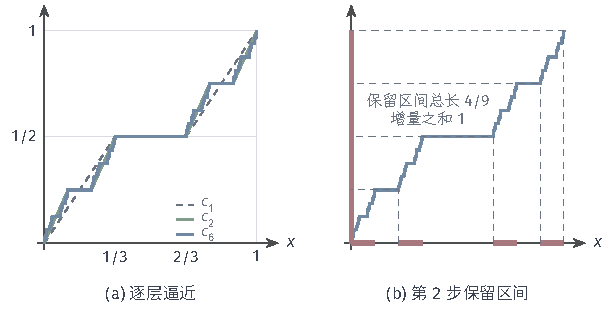
\includegraphics[width=103.847mm]{figures/02-abstract-mathematics/01-metric-and-measure/tikz/c3-cantor-function/figure.pdf}
\caption{Cantor函数及其分段线性逼近。(a)$c_1$（虚线）、$c_2$（绿色）与$c_6$（蓝色），$c_n$在第$n$步的$2^n$个保留区间上线性增加$2^{-n}$，在已删去的区间上保持常值；(b)第二步的四个保留区间$[0,\frac19]$、$[\frac29,\frac13]$、$[\frac23,\frac79]$、$[\frac89,1]$（横轴红色）总长$4/9$，对应的增量（纵轴红色）各为$1/4$，合起来覆盖整个$[0,1]$。}
\label{fig:integral-cantor-function}
\end{figure}

\paragraph{导数读不到的增量}
Cantor集$C$的补集是删去的开区间之并，$c$在其中每个开区间上为常值，所以在$[0,1]\setminus C$的每一点导数为$0$。第二章已经证明$\lambda(C)=0$，因此$c'=0$几乎处处成立，而
\[
 \int_0^1c'(x)\,\mathrm dx=0\ne1=c(1)-c(0).
\]
恢复公式~\eqref{eq:integral-ftc}失败。由定理~\ref{thm:integral-ftc}，$c$不可能绝对连续。这一点也可以直接从定义看出：第$n$步的$2^n$个保留区间（取其内部）两两不交，总长$(2/3)^n\to0$，而$c$在它们上的增量之和始终是$2^n\cdot2^{-n}=1$。所以对$\varepsilon=1$，任何$\delta>0$都会被足够大的$n$打破。

\paragraph{几种性质的比较}
Cantor函数把几种容易混淆的性质分开了。它连续，所以连续不能保证恢复公式；它单调，因而有界变差，并且几乎处处可导，所以这两条也不够；它缺的正是绝对连续性。前面的例子还给出另一侧的分界：$x\sin(1/x)$一致连续却不是有界变差；$\sqrt x$绝对连续却不Lipschitz。概括起来，在$[a,b]$上
\[
 \text{Lipschitz}\Longrightarrow\text{绝对连续}\Longrightarrow\text{连续且有界变差}\Longrightarrow\text{几乎处处可导},
\]
而三个箭头都不能反过来，反例依次是$\sqrt x$、Cantor函数和阶跃函数$\mathbf 1_{[1/2,1]}$（几乎处处可导但不连续）。

Cantor函数那部分导数读不到的增量，正是第二章的奇异连续质量：它没有点质量，却全部集中在零测的Cantor集上（第~\ref{sec:measure-decomposition}节）。一般的有界变差函数，其增量可以分成由导数积分恢复的部分、跳跃部分和这种奇异连续部分；第四章将把函数增量看作测度，用相对于Lebesgue测度的密度重新解释本节的结论。
